\documentclass[aspectratio=169]{beamer}
\usetheme{Madrid}
\usecolortheme{seahorse}
\usefonttheme[onlymath]{serif}
\setbeamertemplate{navigation symbols}{}
\usepackage{amsmath,amssymb}
\usepackage{booktabs}
\usepackage{graphicx}
\usepackage{xcolor}

\title{Seven Recommenders on MovieLens-1M}
\subtitle{Rating prediction and Top-10 recommendation, same split}
\author{Student Name \\ \small NetID@institution.edu}
\institute{CS 550 Massive Data Mining and Learning}
\date{Spring 2026}

\begin{document}

\maketitle

%-----------------------------------------------------------------------------
\begin{frame}{What I built}
  \begin{itemize}
    \item Seven recommender algorithms, one codebase, one split.
    \item Two tasks per the course spec: rating prediction and Top-10.
    \item Everything written from NumPy/PyTorch primitives; no Surprise, no implicit, no lightfm.
  \end{itemize}
  \vspace{0.6em}
  The interesting part is not the numbers on any one model. It is what the comparison tells you about which choices matter.
\end{frame}

%-----------------------------------------------------------------------------
\begin{frame}{Data}
  MovieLens-1M: $1{,}000{,}209$ integer ratings, $6{,}040$ users, $3{,}706$ movies, 20-core on users.
  \begin{itemize}
    \item Drop items with $<5$ ratings to stabilise similarity estimation. Left with $N_u{=}6040$, $N_i{=}3416$.
    \item Per-user hold-out, seed 42: $\approx 800$k train / $200$k test. $95.16\%$ sparse.
  \end{itemize}
\end{frame}

%-----------------------------------------------------------------------------
\begin{frame}{The seven models}
  \small
  \begin{tabular}{lll}
    \toprule
    Group & Model & One-line \\
    \midrule
    Baseline    & GlobalMean    & constant $\mu$ \\
    Baseline    & BiasOnly      & $\mu + b_u + b_i$ by alternating ridge \\
    \midrule
    Memory CF   & ItemKNN       & adjusted cosine, shrinkage, top-50 \\
    Memory CF   & UserKNN       & centred cosine, shrinkage, top-50 \\
    \midrule
    Factor      & MF            & biased SVD, $d{=}64$, Adam, MSE \\
    Neural      & NeuMF         & GMF $\oplus$ MLP, He 2017 \\
    \midrule
    Ranking     & BPR-MF        & pairwise logistic, Rendle 2009 \\
    Graph       & LightGCN      & 3-layer symmetric propagation, He 2020 \\
    \bottomrule
  \end{tabular}
\end{frame}

%-----------------------------------------------------------------------------
\begin{frame}{Evaluation}
  \textbf{Rating.} MAE and RMSE on held-out $(u,i)$ pairs, $\hat r$ clipped to $[1,5]$.\\[0.4em]
  \textbf{Top-10.} For each user: score all items, mask items in training, take top-10, compute P / R / F$_1$ / NDCG against held-out positives. Average over users with $\ge 1$ test item.\\[0.4em]
  BPR-MF and LightGCN produce uncalibrated scores; reporting their MAE/RMSE would be misleading, so those cells are N/A.
\end{frame}

%-----------------------------------------------------------------------------
\begin{frame}{Rating prediction}
  \centering
  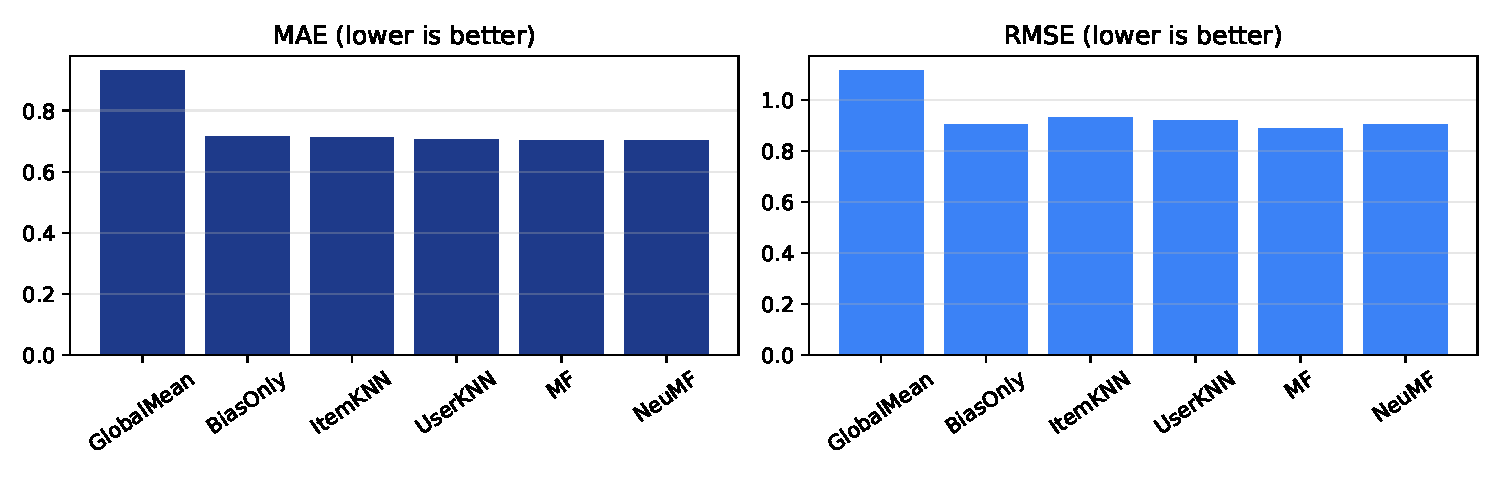
\includegraphics[width=0.92\textwidth]{../results/rating_metrics.pdf}
\end{frame}

%-----------------------------------------------------------------------------
\begin{frame}{Top-10 recommendation}
  \centering
  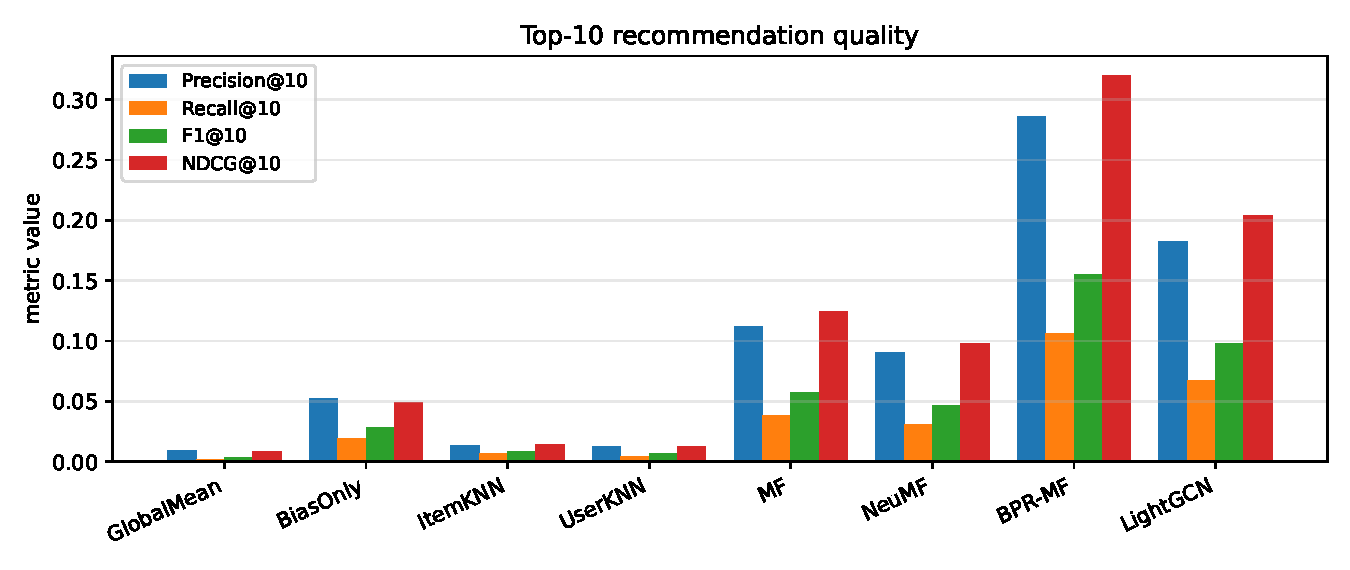
\includegraphics[width=0.98\textwidth]{../results/topn_metrics.pdf}
\end{frame}

%-----------------------------------------------------------------------------
\begin{frame}{Finding 1: the loss matters more than the architecture}
  BPR-MF and MF use the \emph{same} scoring function $p_u^{\top}q_i+b_i$. Only the loss differs.
  \vspace{0.5em}
  \begin{center}\small
  \begin{tabular}{lcc}
    \toprule
    Model & NDCG@10 & P@10 \\
    \midrule
    MF (MSE)       & 0.125 & 0.112 \\
    BPR-MF (BPR)   & \textbf{0.320} & \textbf{0.286} \\
    \bottomrule
  \end{tabular}
  \end{center}
  \vspace{0.5em}
  MSE spends capacity on the 2s and 3s. BPR spends every gradient step on ordering positives above unobserved items, which is what the ranking metrics reward.
\end{frame}

%-----------------------------------------------------------------------------
\begin{frame}{Why kNN is good on rating but bad on ranking}
  UserKNN and ItemKNN match MF on MAE, but trail it by $10\times$ on ranking.
  \vspace{0.3em}

  For unseen items the neighbourhood estimate collapses back to $\bar r_u$: the neighbours that drive the prediction are mostly items the user has already rated, and those are masked out for Top-$N$. The remaining scores stop discriminating.
  \vspace{0.3em}

  Practical fix: use kNN as a candidate generator, then rerank with a ranking model.
\end{frame}

%-----------------------------------------------------------------------------
\begin{frame}{Finding 2: LightGCN does not beat BPR-MF here}
  First run (15 epochs, batch 16k) was much fewer gradient steps than BPR-MF. Easy objection: undertrained. So I reran with matched steps.
  \vspace{0.5em}
  \begin{center}\small
  \begin{tabular}{lrrrr}
    \toprule
    Config & Epochs & Batch & Grad.\ steps & NDCG@10 \\
    \midrule
    LightGCN, short   & 15 & 16{,}384 & $\sim$720   & 0.204 \\
    LightGCN, matched & 20 & 4{,}096  & $\sim$3{,}900 & 0.204 \\
    BPR-MF            & 20 & 4{,}096  & $\sim$3{,}900 & \textbf{0.320} \\
    \bottomrule
  \end{tabular}
  \end{center}
  \vspace{0.5em}
  The matched run gives the same numbers at $46\times$ the wall-clock. The gap is not a compute artefact.
  \vspace{0.3em}

  Most likely cause, by the paper's own Fig.~4: $L{=}3$ is too many layers for ML-1M. The paper's ML-1M optimum is $L{=}2$. I did not sweep $L$.
\end{frame}

%-----------------------------------------------------------------------------
\begin{frame}{Fairness audit}
  If a model funnels every recommendation to the most popular 10 movies, it will look fine on NDCG and terrible on the tail. Worth checking.
  \vspace{0.3em}
  \begin{center}\small
  \begin{tabular}{lrrr}
    \toprule
    Model & Coverage@10 & Gini & Long-tail @10 \\
    \midrule
    GlobalMean & 0.103 & 0.987 & 0.873 \\
    BiasOnly   & 0.095 & 0.995 & 0.260 \\
    ItemKNN    & 0.821 & 0.690 & 0.557 \\
    UserKNN    & 0.757 & 0.749 & 0.870 \\
    MF         & 0.052 & 0.994 & 0.015 \\
    NeuMF      & 0.480 & 0.876 & 0.257 \\
    BPR-MF     & 0.204 & 0.975 & 0.005 \\
    LightGCN   & \textbf{0.022} & 0.995 & \textbf{0.000} \\
    \bottomrule
  \end{tabular}
  \end{center}
  \vspace{0.3em}
  LightGCN's top-10 never leaves the popularity head and touches only 2\% of the catalogue. The two NDCG winners are the two worst on the fairness numbers.
\end{frame}

%-----------------------------------------------------------------------------
\begin{frame}{Web demo}
  Flask + vanilla JS. Pick a user ID, pick a model, get a top-10 list next to that user's top-rated training history. All seven pickled models load at startup; per-user inference is a few milliseconds.
\end{frame}

%-----------------------------------------------------------------------------
\begin{frame}{What I did not do}
  \begin{itemize}
    \item Cold start. Every model is transductive; extending to side information is a separate project.
    \item Temporal dynamics. Timestamps are in the data but the models do not read them.
    \item Layer sweep for LightGCN ($L{=}2$ probably fixes it).
    \item Multiple seeds / bootstrap CIs. Single seed is a rubric weakness.
    \item LLM-based recommenders (P5, SASRec). Adjacent to the spec, not included.
  \end{itemize}
\end{frame}

%-----------------------------------------------------------------------------
\begin{frame}{Bottom line}
  \begin{itemize}
    \item Loss function moved the ranking metrics more than any architectural change.
    \item LightGCN lost on ML-1M under a matched budget; $L{=}3$ is the suspect.
    \item The NDCG winners are also the worst popularity-concentrators. ``Use BPR in production'' is the right first move, not the last.
  \end{itemize}
  \vspace{1em}
  \centering
  Questions?
\end{frame}

\end{document}
